\chapter{\normalfont  INDEL PHASE ANALYSIS VIA THREE PAIRWISE ALIGNMENT METHODS}
\label{ch:three_aln_methods}

\section{Introduction}
The identification and understanding of mechanism behind indel phases is still an unexplored area in molecular and computational biology. Utilizing the correct indel and substitution models more accurately reflects the evolutionary process and leads to fewer biases in phylogenetic inference \parencite{arenas2015trends}. In this chapter, I apply three alignment methods to do our indel phase analysis, including the mafft+sw, coati-max, and coat-sampling alignment, where the latter two utilize the ML estimates from our indel-phase model in chapter 4, to a dataset of 90 species \parencite{zou2021nonsynonymous}. While the mafft+sw approach is a post-alignment correction that searches for the most likely phase of an indel, the coati-max and coati-sampling approaches actively consider gaps within the three indel phases during alignment. The coati-max method searches for the best alignment given the maximum log likelihood, while the coati-sampling method generates all possible alignments with their likelihood in a specified sample size.\\ 
\indent The positive correlation between dN/dS and the ML estimates of $\omega$, and the similar distribution between phase proportions and indel rates across 90 species demonstrate the effectiveness of our indel-phases model. In this chapter, I proposed a new summary statistic – Zn/(Zn+Zs) ratio, which was defined as the number of observed non-synonymous indel events (Zn), in a given evolutionary time, divided by the total number of non-synonymous indel events and synonymous indel events (Zs). \citeauthor{zheng2018correlated} found a strong positive correlation between the deletion events and amino acid replacement in mammalian protein sequences.  Lack of independence between these processes is biologically plausible because natural selection will affect persistence and fixation of both point mutations and insertions or deletions. Besides, our results suggest that the proportion of Zn indels is positively correlated to the ratio of divergence at nonsynonymous and synonymous sites, which can be represented as dN/dS ratio. 


\section{Methods \& Materials}
\subsection{Coati-max \& Coati-sampling Method}
The coati-max is an aligning method built on the Viterbi algorithm, while the coati-sampling is an aligning method built on the Forward algorithm (\href{https://github.com/jgarciamesa/coati}{https://github.com/jgarciamesa/coati}). Both can accommodate different indel phase events. The coati-max method finds the optimal alignment given a pairwise HMMs, and the coati-sampling method averages all possible alignments between the sequence pairs, eliminating bias introduced by the best alignment and allowing the alignment uncertainty to improve the parameter estimates.  

\subsection{Alignment}
Mafft alignment utilized the default parameters and the global alignment algorithm. Coati-max and coati-sampling alignment took advantage of the ML estimates of the indel-phase model from 90 species datasets. Parameters including six $\sigma s, \omega, \tau, g, e$ were utilized as the default parameters for the alignment method. Of note, I took the average of phase 0, phase 1, and phase 2 gap opening weight as g, and the average of insertion and deletion extension weight as e. as the coati methods only accepted one gap opening and one gap extension value. Also, the gap extension weight calculated from the indel-phase model was based on the codon unit, while the calculation from coati aligners was based on a nucleotide unit. Hence, I need to triple the gap length and recalculate the extension weight before using aligners.   

\subsection{Quality Control}
Even though the data was extracted from a published paper \parencite{zou2021nonsynonymous}, I still conducted further data filtering to ensure that the filtered data was suitable for our research goal. Our dataset contained all of the gene pairs instead of a concatenated sequence of each species from chapter 2. I contacted the authors and obtained the aligned coding sequence pairs, removing all aligned gaps to restore the unaligned cds. The main quality control was executed in two-steps: 1) any unaligned sequence with ambiguous nucleotide (N), early stop codons, and in which length were not divisible by three were filtered out; 2) any alignment would be filtered out if they failed our gap-length statistics standard. After I obtained the filtered gene pairs from coati-max, the same gene ID was used to filter out the alignments generated by mafft+sw and coati-sampling methods. \\
\indent Figure 5.1 left displayed a hex plot of one of the species pairs (01\_FcaCaf). Only the gene pairs that satisfy the conditions ($f_{diff}<0.1, f_{adj}<0.5$) remained in the database. The $f_{diff}$ was the percentage of the sequence length difference per gene pair, and the $f_{adj}$ was the penalty of gap per gene pair, which was calculated as $f_{diff} = \mid len_A-len_B \mid/(len_A+len_B)$,  $f_{adj} = (gap.len_A+gap.len_B - \mid len_A-len_B \mid)/(len_A+len_B) $ separately. The threshold value \{0.1,0.5\} was selected based on this empirical data. The complete figure of all 90 species is in APPENDIX \ref{fig:post_fil}. \\ 
\indent Figure 5.1 right was a set of three graphs representing the post-filtering quality of the data. A-plot showed that the evolutionary distance \parencite{erickson2010jukes} per gene pair followed a mixture gamma distribution (components=2) approximately. B-plot displayed that the empirical CDF of the distance followed an uniform distribution roughly, and C-plot was a Q-Q plot between the theoretical CDF and the empirical CDF of the data. 

\begin{figure}[H]
     \centering
     \begin{minipage}[t]{1\textwidth}
     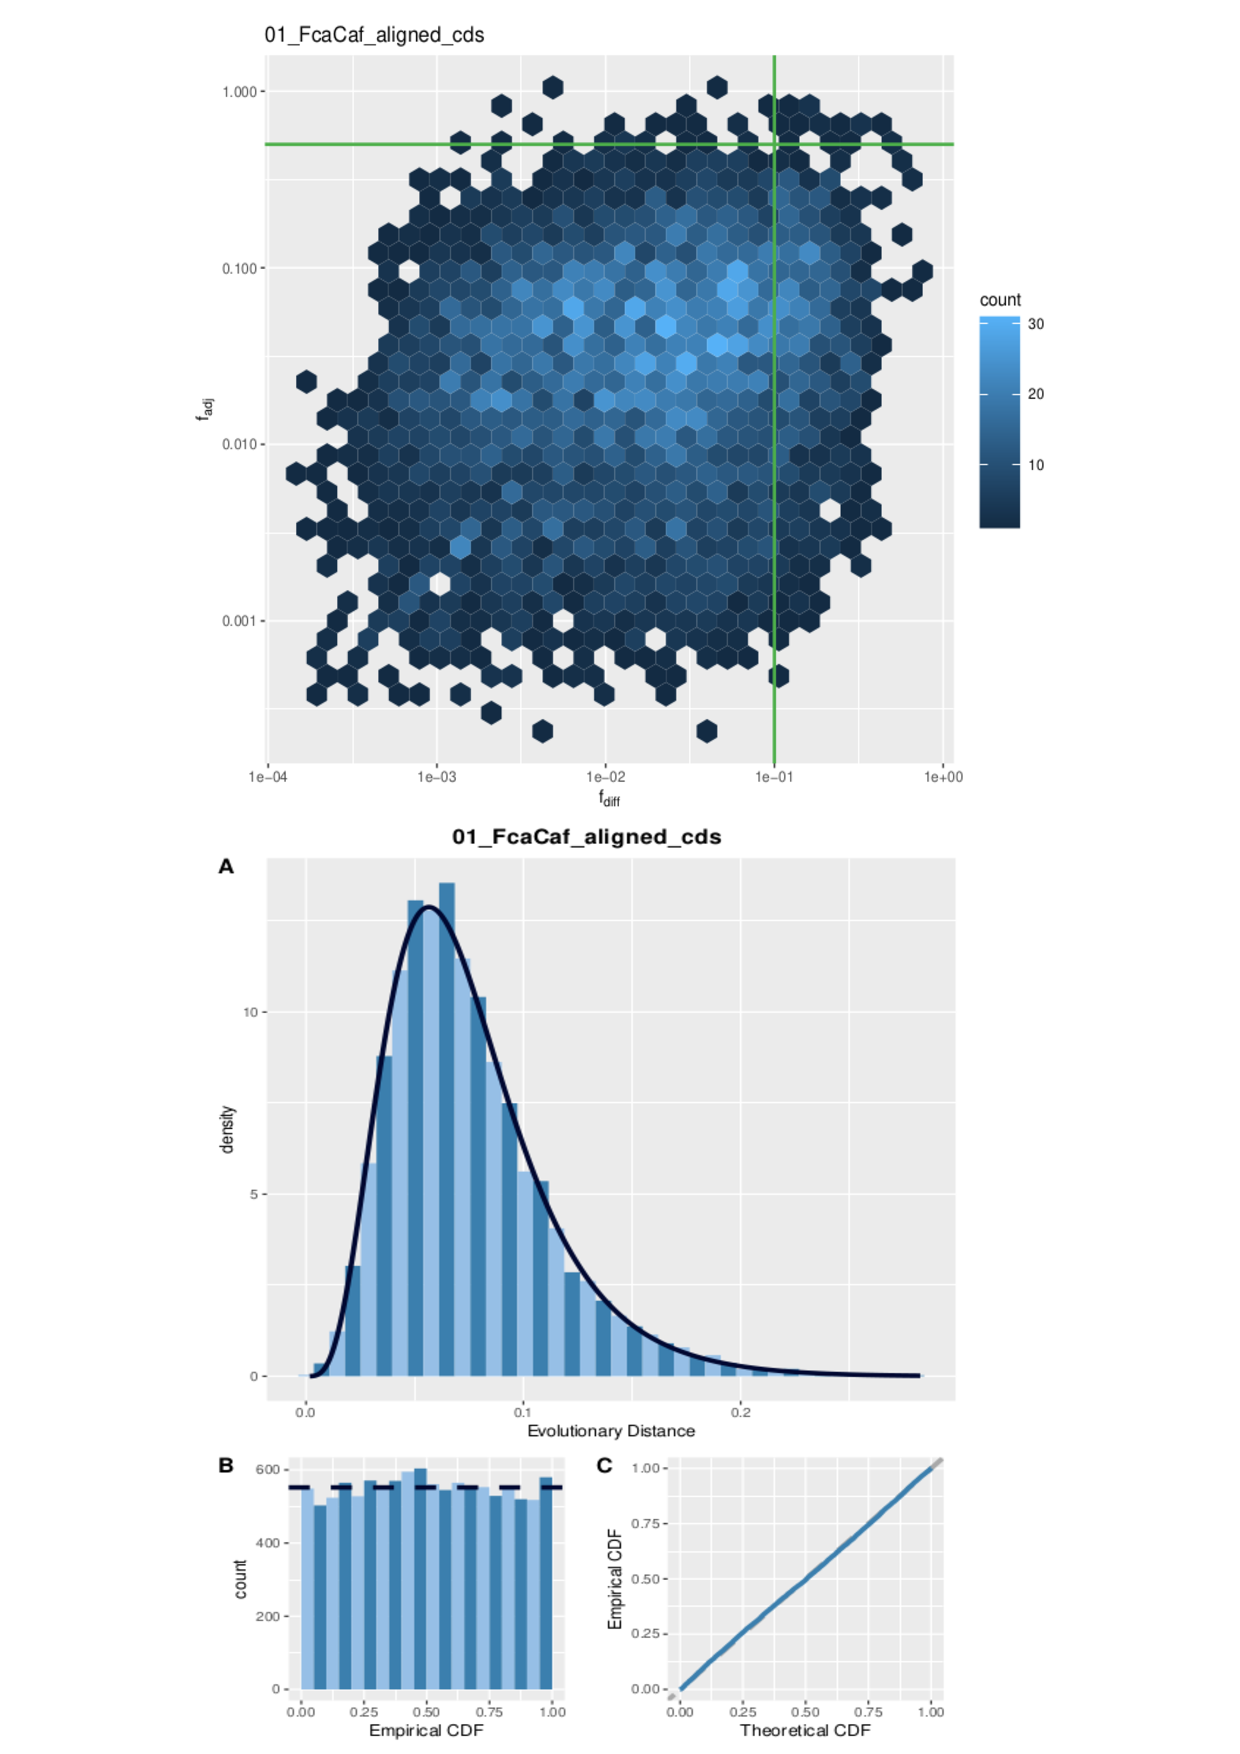
\includegraphics[width=1\linewidth, height=1.3\linewidth]{Fig1.pdf}
     \titlecaption{Quality Control}
      { {Upper figure is the hex plot of one species ($01\_FcaCaf$). $f_{diff}$ is on the x-axis and $f_{adj}$ is on the y-axis. The green line is the threshold. Lower figure is a set of three plots representing the distribution of evolutionary distance.}
      \par}
      \end{minipage}
\end{figure}

\newpage
\subsection{dN/dS vs $\omega$, Phase Proportions vs Normalized Indel Rates}
To test the relationship between our direct summary statistic (dN/dS, phase proportions) and maximum-likelihood estimates ($\omega$, indel rates), I generated a correlation plot between dN/dS and $\omega$, and a distribution plot between phase proportions and normalized indel rates of 90 species across three alignment methods. I normalized the indel rates so that the sum of them equal to 1 so they could compare with the phase proportions. 

\subsection{Indel Phase Proportions across 90 Species}
I extended the phase proportion analysis from mouse-rat species pair to 90 pairwise species spanning over eukaryotes, prokaryotes, and archaea realm. I only applied a single window size (6) on the mafft+sw method. And the coati-max/sampling method automatically generated different indel phases during the alignment. Then I created a table of genome-wide indel phase proportions of each species (APPENDIX \ref{tab:phase_prop_all}), a phase proportion plot across 90 species, and a distribution plot of three indel phases.   

\subsection{dN/dS vs Zn/(Zn+Zs) Ratio}
The dN/dS ratio is commonly used as an indicator of selective pressure acting on a set of homologous protein coding genes. And the interpretation of dN/dS $<$ 1 is implied as negative selection, dN/dS $\sim$ 1 as neutrality, and dN/dS $>$ 1 as positive selection. I measured the dN/dS ratio using the \parencite{nei1986simple} method, 
\begin{gather*} 
\begin{aligned}
 P_n  &= N_d/ N \\
 P_s   &= S_d/S \\
 d_{n}d_{s} &= log(1-4P_n/3)/log(1-4P_s/3) 
\end{aligned}
\end{gather*}
where $N_d$, $S_d$ is the number of observed nonsynonymous, synonymous substitutions, $N,S$ is the number of expected nonsynonymous, synonymous substitutions. Inspired by the formulas above, I proposed a new summary statistic -- Zn/(Zn+Zs) ratio,which was defined as the number of observed non-synonymous indel events ($Z_n$), in a given evolutionary time, divided by the sum of non-synonymous indel events and synonymous indel events ($Z_s$). I generated a distribution plot of dN/dS vs Zn/(Zn+Zs)ratio. The genome-wide ratio across 90 species can be found in APPENDIX \ref{tab:dnds_ZnZs}. \\ 
\indent I investigated the relationship between Zn/(Zn+Zs) vs dN/dS ratio by applying a nonlinear least square fitted function with a logistic regression model, because Zn and Zs followed a binomial distribution with their sum as a weight argument. Next, I generated test data by using the rolling average of their dN/dS and Zn/(Zn+Zs) ratio per 201 gene pairs of each species. The rolling average helps avoid the possibility of zero indel event of any gene pair so the logistic function never collapses. And the total number of rolling average statistics equals the number of gene pairs - 201 + 1 for every species. Next, I was capable of predicting the test data via our nls-logistic model. Besides, I generated several relevant statistics including genome-wide GC percentage, sample size, neutral Zn/(Zn+Zs) value, asymptote and initial slope of our nls-logistic regression function of each species. Notably, neutral Zn/(Zn+Zs) was measured by the deletion of the 3nt gaps in any two codons generated by the empirical frequency from the data. 


%%%%%%%%%%%%%%%%%%%%%%%%%%%%%%%%%%%%%%%%
\section{Results}
\subsection{Compare dN/dS with $\omega$ }
Figure 5.2 presents a positive linear correlation between omega ($\omega$) (ML estimates extracted from GTR+MG94 substitution model) and dN/dS (1989 method) of three alignment methods. The coefficient of determination ($R^2$) of each regression line is around 0.66 which is high, with a small p-value ($\ll 0.05$). The slope of the linear equation of sw, max, and sampling methods is about 1.15, 0.60, 0.60 respectively. The linear regression from the coati-max and coati-sampling method are more similar compared with the mafft+sw method.     
\begin{figure}[H]
     \centering
     \begin{minipage}[t]{1\textwidth}
     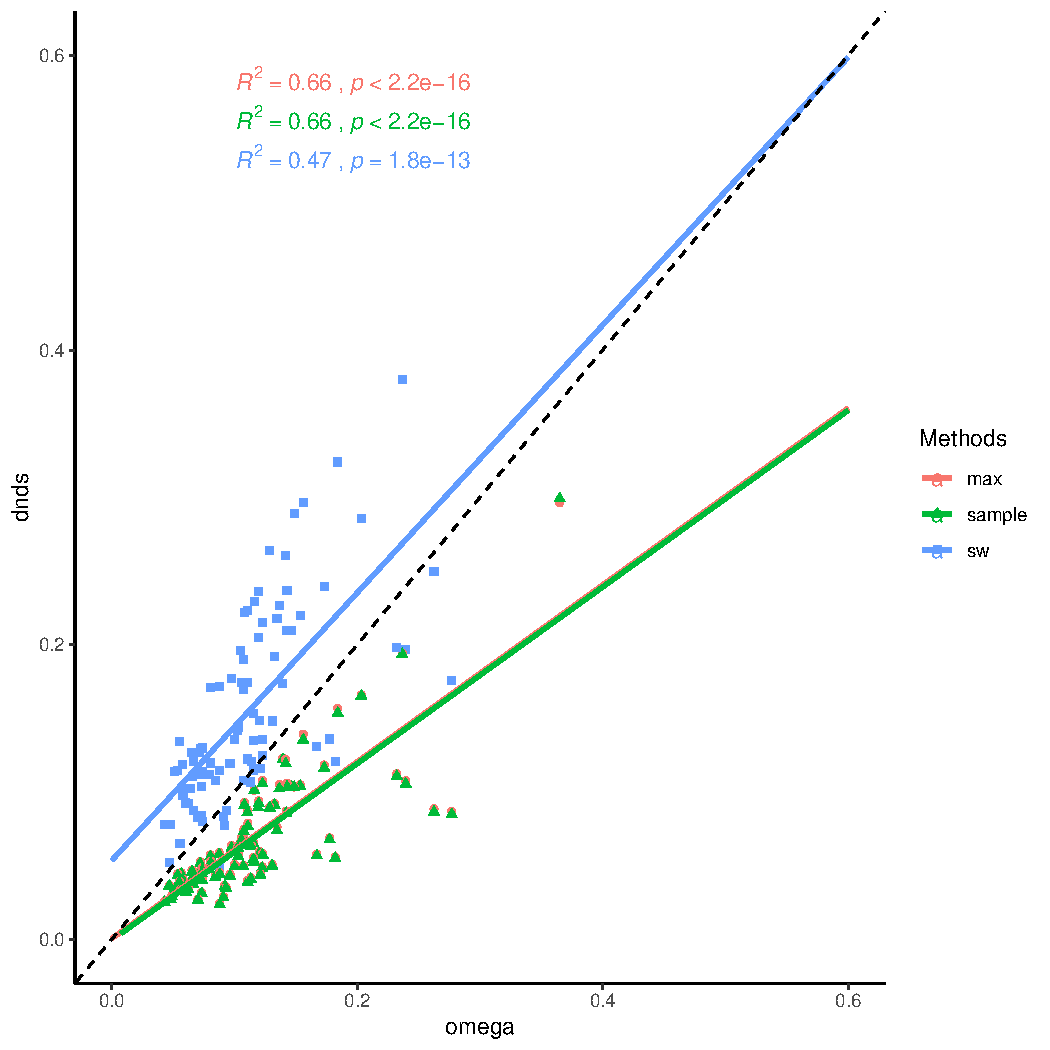
\includegraphics[width=1\linewidth,height=1\linewidth]{Fig2.pdf}
     \titlecaption{Correlation Plot between dN/dS and $\omega$ across 90 Species}
     { {Three linear regression lines describe the relationship between MLE of $\omega$ and dN/dS ratio. The dashed line is a diagonal line with a slope of 1. }
 \par}
     \end{minipage}
\end{figure}

\subsection{Compare Phase Proportions with Indel Rates}
Figure 5.3 compares the distributions between the normalized ML estimate of indel rates and the observed phase proportions across three alignment methods. I found that the distribution of the normalized indel rates displayed a similar trend as the observed proportion of indel phases, which was $r_0 > r_2 > r_1$. Also, the mean value of the phase proportions and the indel rates are very close between the coati-max and coati-sampling method. 
\begin{figure}[H]
     \centering
     \begin{minipage}[t]{1\textwidth}
     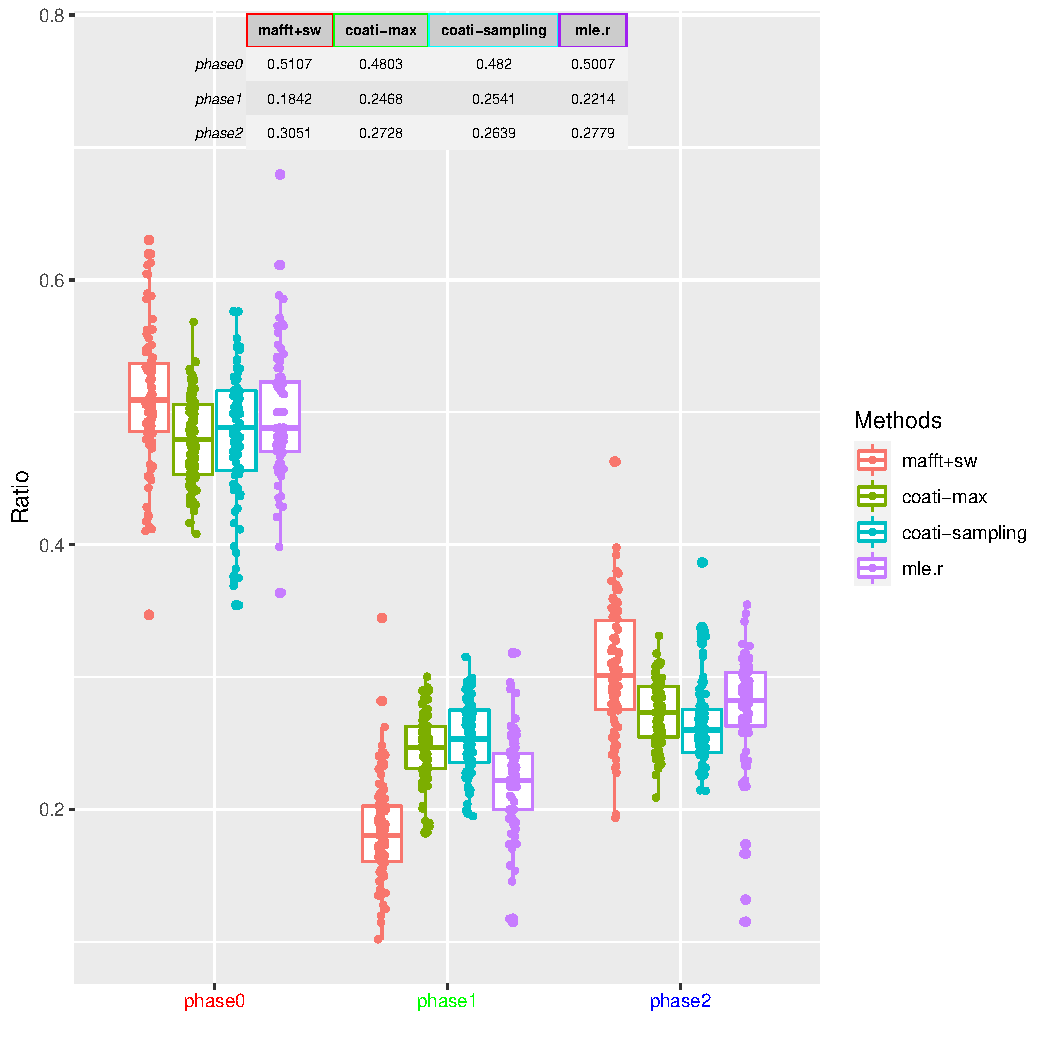
\includegraphics[width=1\linewidth,height=0.9\linewidth]{Fig3.pdf}
     \titlecaption{Distribution Comparison between ML Estimates of Indel Rates and Phase Proportions from Three Methods across 90 Species}
     { {The table represents the mean value of each phase proportions across three alignment methods and the ML estimates of indel rates.}  
 \par}
     \end{minipage}
\end{figure}

\subsection{Phase Proportions across 90 Species}
Figure 5.4 displays the phase proportion histogram of 90 species across three different alignment methods. The phase proportion trend of  $phase 0 > phase 2 > phase 1$ are universal across all of the species regardless of the method. \\
\begin{figure}[H]
     \centering
     \begin{minipage}[t]{1\textwidth}
     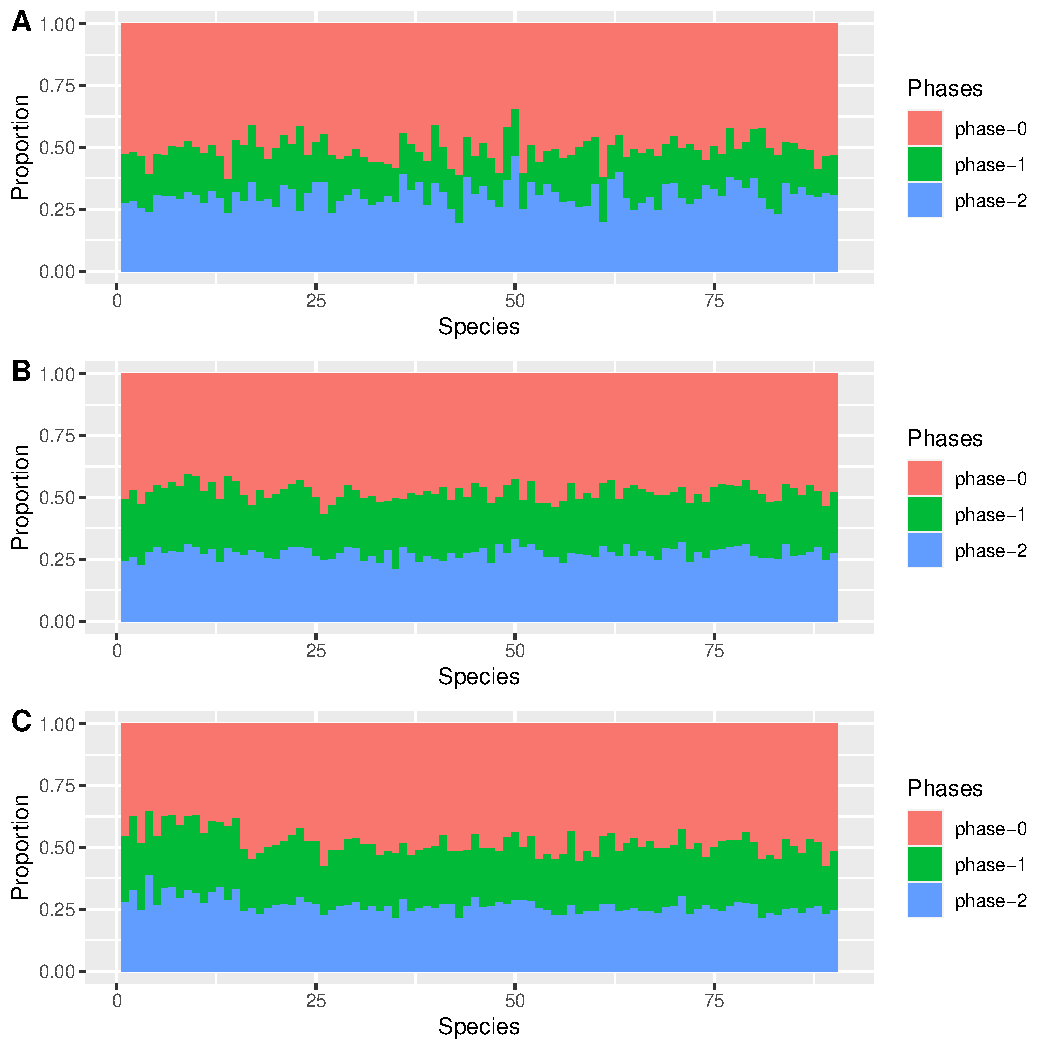
\includegraphics[width=1\linewidth,height=1.1\linewidth]{Fig4.pdf}
     \titlecaption{Phase Proportion Histogram across 90 Species in Three Alignment Methods}
     { {A. mafft+sw. B. coati-max. C. coati-sampling.} 
 \par}
     \end{minipage}
\end{figure}

\indent Figure 5.5 displays the distribution of phase proportions of 90 species across three alignment methods. The genome-wide phase distribution of coati-max and coati-sampling are more similar compared with the mafft+sw distribution.  For example, the mean value of phase 0 proportion of mafft+sw is above 0.5, and the other two are slightly below 0.5. The mean value of phase 1 proportion  of mafft+sw is below 0.2, and the other two are slightly above 0.2. The variance of phase distribution across 90 species is very small ($<0.001$). Besides, I found that the proportion difference between phase 1 and phase 2 are more distinctive in mafft+sw compared to the other two methods. Additionally, the qqplot and shapiro-wilk’s test demonstrated that most of the phase proportions followed a normal distribution except for the phase 0 and phase 2 indels of coati-sampling method and phase 1 indels of mafft+sw method (see APPENDIX \ref{fig:pha_prop}). 
\begin{figure}[H]
     \centering
     \begin{minipage}[t]{1\textwidth}
     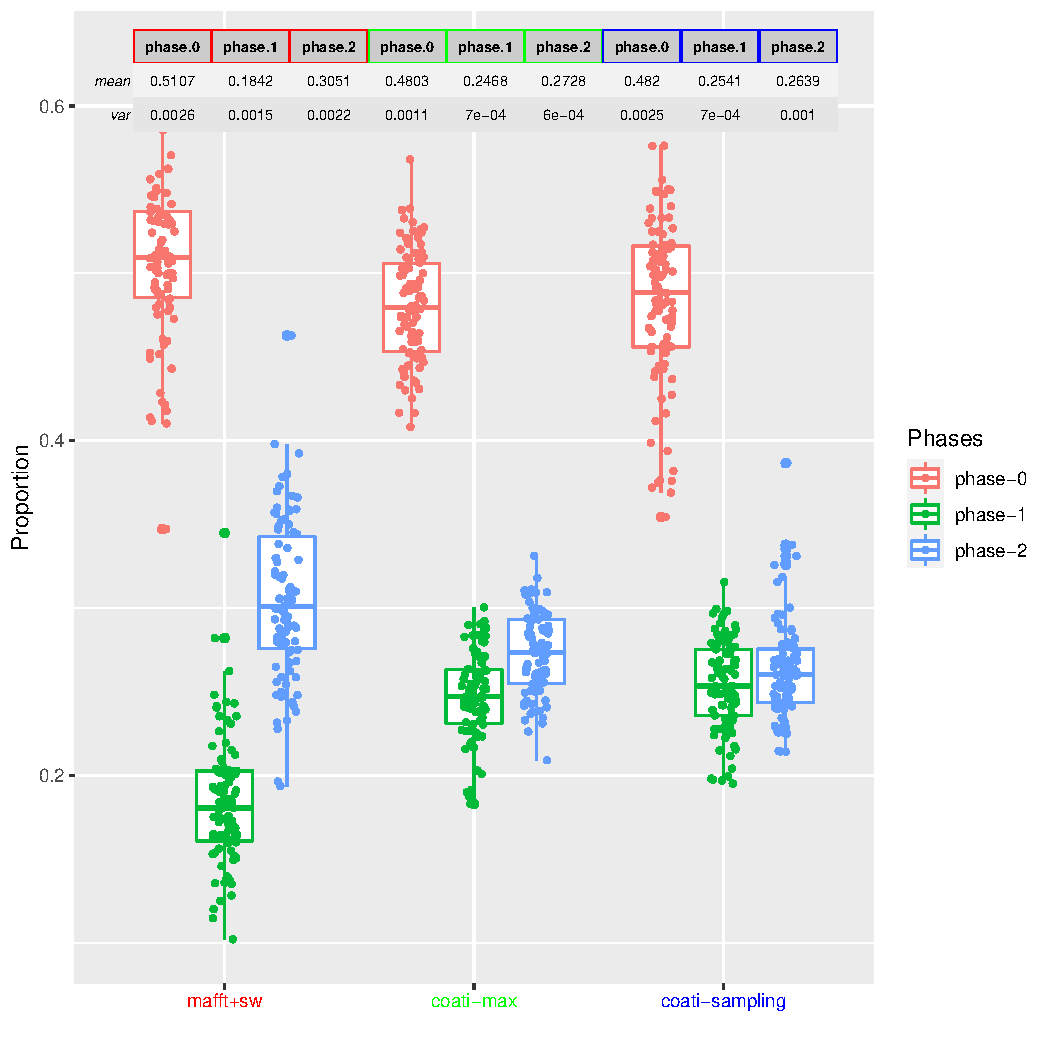
\includegraphics[width=1\linewidth,height=1.1\linewidth]{Fig5.pdf}
     \titlecaption{Phase Proportion Distribution across 90 Species in Three Alignment Methods}
     { { Top: mean/variance table of each indel phase,  red: mafft+sw. green: coati-max. blue: coati-sampling.} 
 \par}
     \end{minipage}
\end{figure}

\subsection{dN/dS and Zn/(Zn+Zs) Distribution}
Figure 5.6 displays the genome-wide distribution of dN/dS and Zn/(Zn+Zs) ratio of 90 species across three alignment methods. I found that the total number of indels from mafft+sw method are far less than the one from the other two methods. A general trend of larger proportions of Zs indels displays in every species. The upper figure shows a general pattern of dN/dS ratio that is smaller than the Zn/(Zn+Zs) ratio across three alignment methods. The dN/dS distribution is positively skewed which suggests their mean is greater than the mode, while the Zn/(Zn+Zs) distribution is negatively skewed, which suggests their mean is less than the mode.\\
\indent Additionally, the mean and variance of dN/dS and Zn/(Zn+Zs) ratio are closer in coati-max and coati-sampling methods. The lower figure displays the difference of Zn/(Zn+Zs) value between any two methods. Although the paired-sample wilcoxon signed rank test rejected the null hypothesis ($<0.05$) that the median of the population of differences between the paired data is zero, the comparatively large p-value from coat-max/sampling group indicated their data similarity. 
\newpage
\begin{figure}[H]
    \vspace*{-0.5in}
     \centering
     \begin{minipage}[t]{1\textwidth}
     \centering
     \includegraphics[page=2,width=0.7\linewidth,height=0.6\linewidth]{Fig6.pdf}
     \includegraphics[page=3,width=0.7\linewidth,height=0.6\linewidth]{Fig6.pdf}
     \titlecaption{Genome-wide Distribution of Zn/(Zn+Zs) Value.}
     { {Upper: genome-wide distribution of dN/dS and Zn/(Zn+Zs) value of 90 species across three alignment methods (top: mean/variance table of dN/dS and Zn/(Zn+Zs) value). Lower: Zn/(Zn+Zs) ratio comparison between methods, p value is calculated from the Wilcoxon signed rank test.}
     \par}
     \end{minipage}
\end{figure}

\subsection{The Relationship between dN/dS and Zn/(Zn+Zs)}
Figure 5.7 displays a relationship between dN/dS and Zn/(Zn+Zs) ratio of two of 90 species (05\_Droso, 10\_ants). The upper figure displays a positive change of rolling average of Zn and Zs per 201 gene pairs with the increment of the dnds value. The lower figure presents a positive correlation between Zn/(Zn+Zs) and dN/dS rolling ratio. While the response value approximates the asymptote when the dN/dS ratio increases, the asymptote value is still lower than the neutral Zn/(Zn+Zs) value in most of our species. Besides, although a positive correlation between dN/dS and Zn/(Zn+Zs) exist in most species, there are a few exceptions whose initial slopes are negative or near zero, in which their sample size are too small to support our model, such as ATGC138, ATGC246, and ATGC260. The complete correlation figure of 90 species can be found in Appendix \ref{fig:dnds_ZnZs_corr}.  
\begin{figure}[H]
     \begin{subfigure}[b]{0.5\textwidth}
      \centering
     \includegraphics[page=4,width=1\linewidth,height=1.2\linewidth]{Figure/roll_ZnZs_max.pdf}
     \end{subfigure}%
     \begin{subfigure}[b]{0.5\textwidth}
      \centering
     \includegraphics[page=9,width=1\linewidth,height=1.2\linewidth]{Figure/roll_ZnZs_max.pdf}
     \end{subfigure}
     \titlecaption{Correlation Plot between dN/dS and Zn/(Zn+Zs) Ratio of Drosophila and Ant Species.}
     { {Upper: Each line represents the rolling mean of Zn and Zs value. Lower: a nonlinear red line represents the correlation between Zn/(Zn+Zs) and dN/dS values. Upper left of the figure: genome-wide GC percentage, sample size -- the number of gene pairs, neutral Zn/(Zn+Zs) is measured using the expected number of Zn and Zs value; asymptote line represents the maximum value of Zn/(Zn+Zs) when dN/dS increases to 1, $\tau$ is the branch length, init-slope represents the initial slope of the nonlinear model, and r is the Pearson correlation coefficient.}
     \par}
\end{figure}
\newpage

%%%%%%%%%%%%%%%%%%%%%%%%%%%%%%%%%%%%%%%
\section{Discussion}
The correlation between $\omega$ and dN/dS ratio, distribution similarity between indel rates and phase proportions suggested the effectiveness of our indel-phase model on the real sequence data. The indel phase proportion results demonstrated an universal purifying selection effect on the genomic coding regions of 90 species pairs regardless of the alignment methods. The similarity of phase proportions, dN/dS ratio, and Zn/(Zn+Zs) distributions between coati-max and coati-sampling was attributed to their model resemblance, which is different from the mafft+sw method. The positive correlation between Zn/(Zn+Zs) and dN/dS ratio showed a great potential of using Zn/(Zn+Zs) as an alternative indicator of natural selection.

\subsection{dN/dS vs $\omega$, Phase Proportions vs Indel Rates}
There is a linear correlation between the dN/dS ratio and the ML estimates of $\omega$ of 90 species across three alignment methods. This consistency demonstrated the accuracy of our model on estimating parameters. Since the measure of dN/dS ratio required the observed non-synonymous over synonymous ratio normalized by the expected non-synonymous over synonymous ratio, which was different from the way of estimating the $\omega$ from the EM method. Besides, we found that the lowest R-squared value from the mafft+sw method was likely due to the less amount of data compared with the coati-max and coati-sampling method. \\
\indent While there is not an obvious linear correlation between the phase proportions and ML estimates of indel rates, which is mostly likely due to the lack of sufficient gap events compared to the substitutions. Still, our distribution results suggested that the three normalized indel rates displayed the same trend as the phase proportions across three methods ($phase 0 > phase 2 > phase 1$).    

\subsection{Zn/(Zn+Zs) vs dN/dS ratio}
The positive correlation between Zn/(Zn+Zs) and dN/dS ratio suggested that I could predict them with a nonlinear function. While a few species with a smaller sample size displayed a negative initial slope, most of their initial slopes were positive with a high Pearson correlation coefficient. Besides, I found that the closer two species are, the harder it is to get good estimates of the correlation function due to the fewer Zn and Zs events. For example, 05\_droso and 10\_ants both belong to the insect branch, while the former displays a flat curve that might be attributed to its lower branch length. Moreover, I found that the 06\_nematode displayed a reduction in Zn and Zs after reaching the peak might be an artifact due to its large divergence($>1$). Additionally, I realized that the little change of Zn/(Zn+Zs) normally required a big change of dN/dS value in our 90 species dataset. While this correlation limited to the indel size of 3,6,9,12 np, the universal positive relationship within our dataset was non negligible. 